\documentclass{article}

\usepackage[utf8]{inputenc}
\usepackage{graphicx}
\usepackage{geometry}
\usepackage{caption}
\usepackage[romanian]{babel}
\usepackage{xcolor}
\usepackage{listings}


\definecolor{mGreen}{rgb}{0,0.6,0}
\definecolor{mGray}{rgb}{0.5,0.5,0.5}
\definecolor{mPurple}{rgb}{0.58,0,0.82}
\definecolor{backgroundColour}{rgb}{0.95,0.95,0.92}

\lstdefinestyle{CStyle}{
	backgroundcolor=\color{backgroundColour},   
	commentstyle=\color{mGreen},
	keywordstyle=\color{magenta},
	numberstyle=\tiny\color{mGray},
	stringstyle=\color{mPurple},
	basicstyle=\footnotesize,
	breakatwhitespace=false,         
	breaklines=true,                 
	captionpos=b,                    
	keepspaces=true,                 
	numbers=left,                    
	numbersep=5pt,                  
	showspaces=false,                
	showstringspaces=false,
	showtabs=false,                  
	tabsize=2,
	language=C
}


\providecommand{\keywords}[1]{\textbf{\textit{Keywords -}} #1}



\geometry{
	a4paper,       
	textwidth=14cm,  
	textheight=23cm,
	heightrounded,   
	hratio=1:1,    
	vratio=2:3,     
}



\title{mySSH}
\author{Milea Mihai-Cristian}


\renewcommand*\contentsname{Cuprins}
\renewcommand{\figurename}{Fig.}

\begin{document}
	\begin{titlepage}
		
		\newcommand{\HRule}{\rule{\linewidth}{0.5mm}} 
		
		\center 
		\vspace*{\fill}
		
		\textsc{\LARGE Universitatea „Alexandru Ioan Cuza”\newline Facultatea de Informatiă}\\[1.5cm] 
		\textsc{\Large Rețele de Calculatoare}\\[0.5cm] 
		
		\HRule \\[0.4cm]
		{ \huge \bfseries MySSH }\\[0.4cm] 
		\HRule \\[1.5cm]
		
		
		
		\begin{minipage}{0.4\textwidth}
			\begin{flushleft} \large
				\emph{Autor:}\\
				Milea \textsc{Mihai-Cristian I2A4} 
			\end{flushleft}
		\end{minipage}
		~
		\begin{minipage}{0.4\textwidth}
			\begin{flushright} \large
				\emph{Coordonator:} \\
				Colab. Stănescu \textsc{Ioana} 
			\end{flushright}
		\end{minipage}\\[2cm]
		\keywords{
			\centering SSH · TCP · IP · client-server · securitate · criptare · socket · fork
		}
		\newline
		
		
		{\large \today}\\[1cm] 
		
		\vfill
		
	\end{titlepage}
	\newpage
	
	\pagenumbering{arabic}
	\tableofcontents
	
	\newpage
	\section{Introducere}
	
	\paragraph {
		SSH = Secure Socket Shell\\
		Protocoalele SSH1 și SSH-1 au fost developate in 1995 de către Tatu Ylönen, un cercetător de la universitatea de tehnologie in Helsinki, Finlanda.\\
		Modelul său SSH-1 a început să capete din ce in ce mai multă atenție. Cu timpul și-a dat seama că produsul său poate fi utilizat în multe moduri.\\
		In Iulie 1995, SSH-1 a fost disponibil ca software gratuit cu tot cu cod sursă, ca să poate fi copiat și utilizat de oricine și-ar fi dorit.\\
		Până la finalul anului 20.000 de utilizatori din 50 de țări diferite au adoptat SSH-1. Ylönen primea câte 150 de mesaje pe e-mail de la utilizatori cerând suport.
		\\
		Cu timpul a fost înbunătățit. În acest proiect sunt implementate aceleași idei pe care le-a avut si Ylönen. 
		Scopul este realizarea comunicării mai multor utilizatori cu un server. \\
		Exemplu: PuTTY\\
		Conținutul lucrarii prezintă schimbul de informații criptate între server și utilizatori.
		}

	\paragraph{
		Acest proiect funcționează pe baza protocolului TCP/IP prin care un utilizator se conectează inițial la un server cu credențialele sale de mySSH, având ulterior posibilitatea de a face uz de comenzile pe care le are la dispoziție (date de server).
	}
	\section{Despre mySSH}
	\paragraph{
		Modelul implementat în acest proiect are ca scop interpretarea comenzilor de către server și execuția comenzilor cerute de către utilizatori. Utilizatorii sunt identificați printr-un fișier cu conținut criptat. Utilizatorii pot trimite comenzi către server iar acesta va trimite înapoi execuția.
	}
	\paragraph{
		Cerință: Sa se implementeze o pereche client/server capabila de autentificare si comunicare encriptate. Server-ul va executa comenzile de la client, si va returna output-ul lor clientului. Comenzile sunt executabile din path, cu oricat de multe argumente; cd si pwd vor functiona normal. Se pot executa comenzi multiple legate intre ele sau redirectate prin: \textbar. \textgreater, \textless, 2\textgreater, \&\&, \textbar\textbar, ;.
		\newline
		Această cerință induce la crearea unui server iterativ. Metoda abordată în acest proiect este următoarea: rezervarea a câte un proces pentru fiecare utilizator.
	}
	
	\newpage
	\section{Tehnologii utilizate}
	\paragraph{
		Pentru realizarea acestui proiect au fost utilizate protocolul TCP/IP pentru stabilirea conexiunii între client și server.
	}
	
	\subsection{TCP/IP}
	
	\paragraph{
		Modelul TCP/IP este cel mai utilizat model pentru comunicarea dintre
		calculatoare. Denumirea sa provine de la cele două protocoale fundamentale
		utilizate: TCP (Transmission Control Protocol) şi IP (Internet Protocol).
	}
	
	\paragraph{
		Protocolul TCP este un protocol orientat-conexiune sigur ce permite transmiterea unui flux de octeți de la o mașina la alta fara erori, astfel vor exista pierderi de informație. Pentru fiecare pachet IP trimis, se așteaptă o confirmare că pachetul a fost trimis. Dacă dupa un anumit interval de timp acest răspuns nu apare, atunci pachetul va fi retrimis.
	}
	\paragraph{
		Deasemenea, la recepţionare se verifică integritatea datelor, în cazul în care datele au fost afectate se cere retransmiterea mesajului.
		Unele pachete pot ajunge înaintea altora și pot avea alte topologii de a-și face drum la destinație.
	}
	\begin{figure}
		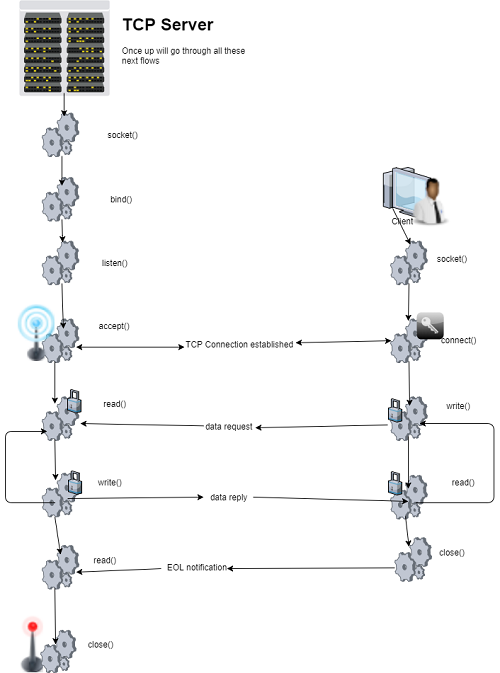
\includegraphics{tcpip}
	\end{figure}	
	

	
	\newpage
	\section{Arhitectura Aplicatiei}
	
	\paragraph{
		Proiectul este împărțit în doua aplicații ce pot fi configurate independet. De pilda, se pot modifica proturile pe care se realizează comunicarea între server si clienți. De menționat este că numărul de utilizatori pe care îî poate susține aplicația server depinde de capacitatea mașinii. De asemenea, numarul maxim de utilizatori din fișierul de utilizatori este de 64, și el modificabil.	
	}
	\paragraph{
	Odata ce serverul va porni, se va alfa intr-o stare blocantă până la stabilirea conexiunii cu un client. Această conexiune se realizează într-un proces copil. După care procesul rădăcina va reintra iar in aceeași stare. Transferul de date se face cu o cheie de criptare privată. Dacă comanda introdusă de client este diferită, va fi tratată într-un mod diferit. Pentru manevrarea mai ușoară a comenzilor primite de către clienți, odată ce au drepturi, ele sunt sparte în cuvinte, utilizate ulterior. Un utilizator are la dispoziție 3 greșeli de autentificare. Dacă datele introduse sunt greșite, la a 3-a incercare nereușită se va încheia legatura dintre server și client.
	}
	
	\subsection{Client}
	\paragraph{
		Prima parte a acestui proiect este aplicația Client. Aceasta îi va permite utilizatorului să se conecteze la server printr-un IP si un port, inserate de către utilizator. Utilizatorul se va afla in 3 etape de-a lungul utilizării aplicației Client din perspectiva aplicației Server.
	}
	\paragraph{Pasul I - Introducerea username-ului. Dacă va fi găsit se va trece la pasul II, daca nu, se repetă pasul I;}	
	\paragraph{Pasul II - Introducerea parolei username-ului. Daca parola introdusă coincide cu cea a username-ului atunci se va trece la pasul III, daca nu, se repetă pasul II;}
	\paragraph{Pasul III - Clientul poate utiliza toate funcțiile pe care i le pune la dispoziție serverul;}		
	
	
	\paragraph{
		Printre caracteristicile aplicației Client se numară:
	}
	
	\begin{itemize}
		\item linie de comandă;
		\item utilizarea comenzilor specifice;
		
		
		
	\end{itemize}
	
	\paragraph{
		O listă a acțiunilor ce pot fi executate de către utilizator in cadrul serverului u o scurtă descriere, este reprezentată în tabelul de mai jos
	}
	\begin{center}
		\begin{tabular}{|l|p{12cm}|}
			\hline
			\textbf{\textit{Comamndă}} & \textbf{\textit{Descriere}} \\ \hline
			help & Afișează o listă a comenzilor. \\ \hline
			cd & Modifica directorul pe care se afla utilizatorul. \\ \hline
			disconnect & Încheie conexiunea cu serverul. \\ \hline
			dir & Afișează conținutul folderului aflat pe server.\\ \hline
			pwd & Afișează path-ul curent. \\ \hline
			mv & Mutarea unui fișier dintr-un loc in altul.\\ \hline
			mkdir & Crează un director nou. \\ \hline
			rmdir & Ștergerea unui folder. \\ \hline
			rm & Ștergerea unui fișier aflat pe server. \\ \hline
			ls & Afișează o listă a fișierelor și a folderelor aflate în folderul curent. \\ \hline
			wget & Descarcă un fișier. \\ \hline
			echo & afișează o secvență de caractere.\\ \hline
			who & Listează utilizatorii conectați, de când sunt conectați si adresele fiecăruia. \\ \hline
			mcedit & Permite editarea unui fișier cu editorul McEdit. \\ \hline
			nslookup & Afișează informatii despre un hostname. \\ \hline
			pwd & Afișează folderul curent de lucru de pe server. \\ \hline
			touch & Creează un fișier. \\ \hline
			zip/unzip & Arhivează sau dezarhivează un set de fișiere respectiv o arhivă. \\ \hline
			chmod & Modifică atributele unui fișier (drepturi).\\ \hline
			cp & Copiază un fișier intr-o altă locație. \\
			\hline
		\end{tabular}
	\end{center}
	\paragraph{Serverul acceptă și comenzi înlănțuite: ls -a \textgreater  intro.txt}
	
	
	\subsection{Server}
	
	\paragraph{
		A doua parte a acestui proiect constă în aplicația Server, care se va afla pe calculatorul ce se dorește a fi utilizat drept gazdă pentru Clienți. Câteva din funcțiile pe care le dispune această aplicație:	
	}
	
	\begin{itemize}
		\item criptarea traficului dintre client și server;
		\item implementarea comenzilor ce permit administrarea serverului de la distanță;
		\item filtrarea IP-urilor, permite verificarea adresei IP de la care se conectează utilizatorul și stabilește dacă aceasta este una autorizată sau nu;
		\item implementarea unui sistem de autorizare de tipul whitelist\textbackslash blacklist pentru conturile utilizatorilor.
	\end{itemize}
	
	\subsection{Stabilirea Conexiunii}
	
	\paragraph{
		În continuare vom trage o ochiadă asupra conexiunii ce urmează să se stabilească între calculatorul nostru - \textit{Clientul} - și calculatorul gazdă, cu care dorim să comunicăm - \textit{Serverul}.
	}

	
	\paragraph{
		În momentul în care s-a realizat conexiunea clientul este pus in pasul I. Conexiunea se va face printr-un port prestabilit pe portul 6636, iar daca se dorește se poate face și pe alt port.
	}
	
	\graphicspath{C:/Users/Zap/Desktop/}
	\begin{figure}
		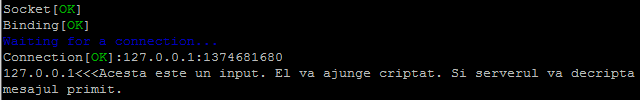
\includegraphics[scale=1]{server}
	\end{figure}
	
	
	\subsection{Procesarea Comenzilor}
	\begin{figure}
		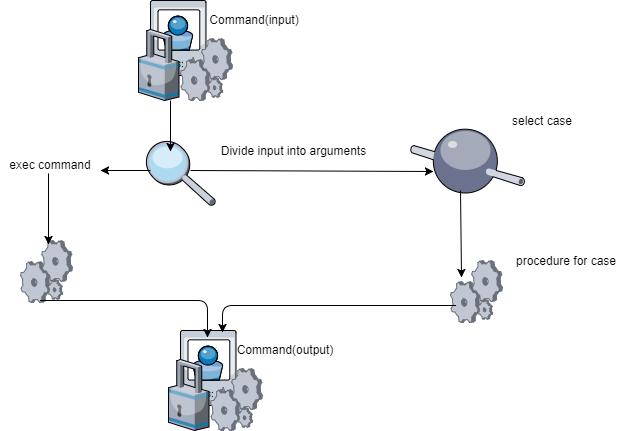
\includegraphics[scale=0.7]{srvcore}
	\end{figure}
	
	
	\begin{lstlisting}[style=CStyle]
	struct mySSH_user{
	char username[20]; 	//numele utilizatorului
	char passwd[20];   	//parola utilizatorului
	int id;				    	//id-ul utilizatorului
	};
	\end{lstlisting}
	Informațiile expuse mai sus sunt salvate si păstrate criptate. De exemplu
	\paragraph{
		Procesarea comenzilor se va realiza atât de partea aplicația client cât și de aplicația server, ambele părți efectuând acțiunile aferente comenzii inițiate.	Unele comenzi trebuiesc tratate în mai multe runde. De exemplu dacă se dorește editarea unui fișier acesta va fi salvat local, editat local și încărcat inapoi in calculatorul gazdă. Altele vor fi tratate intr-o singura rundă. De exemplu afișarea fișierelor din directorul curent. Fiecare utilizator va fi stocat in server cu informațiile acestuia. 
	}
	
	
	
	
	\newpage
	\subsection{Securitate}
	
	\paragraph{
		Orice transfer de date între server si client se face protejat. Pentru că se bazează pe clienți, există vulnerabilitate. Un exemplu ar fi un SMBbomb, unde serverul va primi nenumărate conexiuni până nu mai face față.
		\\Unele din atacurile pe care le poate suferi serverul:
	}
	\begin{itemize}
		\item Atacurile de tip Brute force
		\item Captura de pachete
		\item Atac de tip Spoofing
	\end{itemize}
	
	\paragraph{
		O metodă bonus pentru a securiza transferul de date ar fi:
	}
	\begin{itemize}
		\item Utilizarea unei rețele private (VPN).
		 
	\end{itemize}
	
	
	
	

	
	\section{Server-core}
	
	\paragraph{Serverul va primi de la client o comandă și serverul trebuie sa interpreteze comanda și să îi returneze ce va afișa execuția. Pentru acest lucru se va crea un nou proces copil. Se va duplifica afișarea execuției într-un buffer trimis mai apoi la client.\\
	}

	
	

	\newpage
	\section{Concluzii}
	\paragraph{
	Acest proiect va dispune un set de aplicații (client/server) de comunicare a mai multor clienți cu un server. Aceasta soluție poate fi înbunătățită printr-un algoritm de criptare de genul RSA, SSL și o interfată grafică prietenoasă.	
	}
	\newpage
	\section{Bibliografie}
	
	\begin{enumerate}
		\item http://slacksite.com/other/ftp.html
		\item http://www.unixinside.org/projects/linux-ro/RFC/rfc959-ftp.html
		\item https://docstore.mik.ua/orelly/networking\_2ndEd/ssh/ch01\_05.htm
		\item https://profs.info.uaic.ro/~computernetworks/files/NetEx/S9/servTcpCSel.c
		\item http://www.cs.rpi.edu/~moorthy/Courses/os98/Pgms/socket.html
	\end{enumerate}
	
\end{document}